\section{Durchführung}
\label{sec:Durchführung}
%@Rene: Wenn dir ein besserer Name als "Schaltplatte" einfällt, kannst du diesen gerne ersetzen xD

Alle Messungen werden mit der in \ref{fig:platte}
gezeigten Schaltplatte durchgeführt. 
\begin{figure}
    \centering
    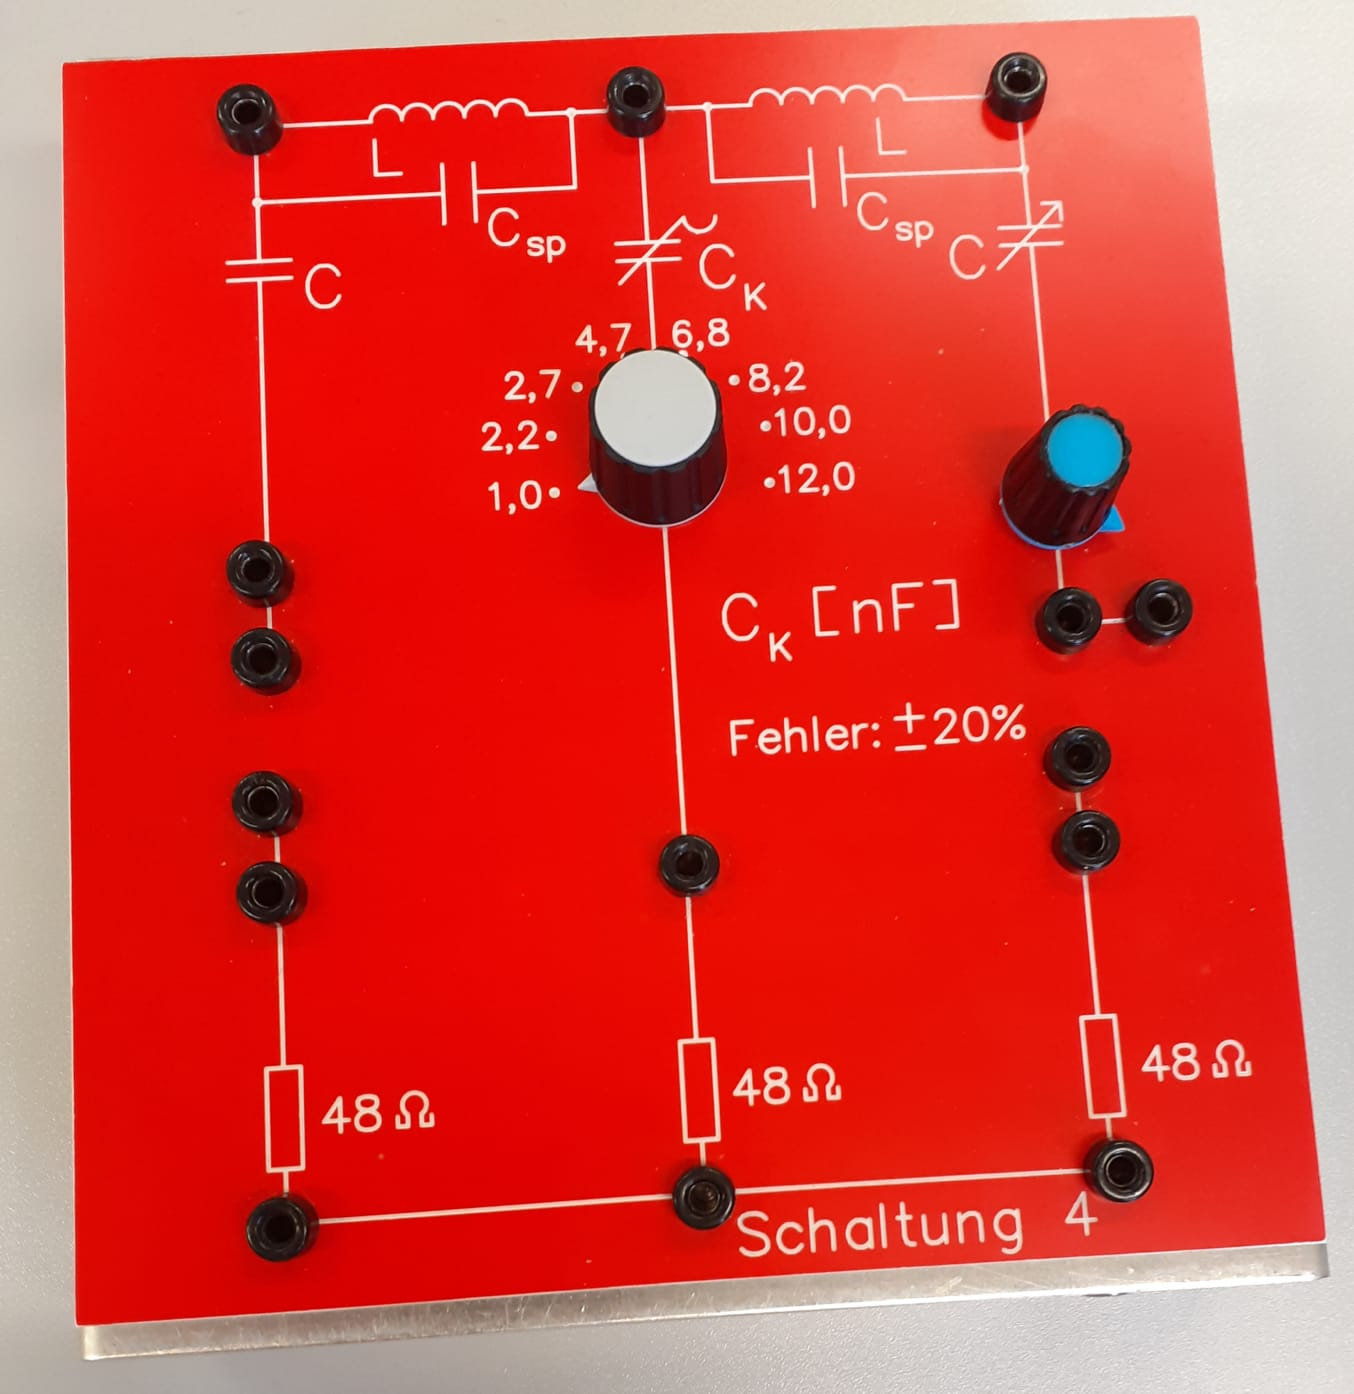
\includegraphics[width=0.5\textwidth]{plots/Platte.jpeg}
    \caption{Die verwendete Schaltplatte.}
    \label{fig:platte}
\end{figure}

\subsection{Vorbereitung: Einstellung der Kapazität}
Damit ein Energieaustausch wie in \ref{sec:Theorie} möglich ist, müssen beide Schwingkreise die gleiche Resonanzfrequenz 
aufweisen. 
Deshalb wird im Folgenden die Resonanzfrequenz des einen Schwingkreises mit fester Induktivität und fester Kapazität bestimmt 
und im Anschluss die Messung an dem zweiten Schwingkreis wiederholt -- mit dem Unterschied, dass hier die regelbare Kapazität so
eingestellt wird, dass die gleiche Resonanzfrequenz gemessen werden kann. 

%%%%%%%%%%%%%
%%HIER Schaltplan wie in Abb. 5 einfügen
%%%%%%%%%%%%%%%%%%%
Die Schaltung wird gemäß (HIER Referenz zur Abbildung hinzufügen) aufgebaut. 
Die Resonanzfrequenz liegt an, wenn im XY-Betrieb des Oszillographen die zu einem Phasenunterschied von $\sfrac{\pi}{2}$ 
gehörige Lissajous-Figur --  also ein Kreis -- erkennbar wird.

%%%%%%%%%%%%%%%%%%%%%%%%%%%%%%%%%%%%%%%%%%%%%%%%%%%%%%%%%%%%%%%%%%%%%%%%%%%%%%%%%%%%%%%%%%%%%%%%%%%%%%%%%%%%%%%%%%%%%%%
\subsection{Messprogramm}
%%%%%%%%%%%%%%%%%%%
%%HIER schaltpülan einfügen wie Abb. 6
%%Nur statt 50 Ohm => 48 OHM
Zuerst wird der Schaltplan gemäß <Hier referenz zu Schaltplan einfügen> aufgebaut. 
Der linke Schwingkreis soll hier über ein Rechteck-Signal des Sinus-Generators angeregt werden. 
Zum rechten Schwingkreis gelangt die Schwingungsenergie demnach ausschließlich über die gemeinsame Kopplungsleitung. 
Die über den Widerstand abfallende Spannung wird über den Y-Eingang an dden Oszillographen gegeben. 
Dort kann jetzt der zeitliche Schwingungsverlauf der Spannung verfolgt werden. 
Von Interesse sei hier das Verhältnis von Schwingungs- zu Schwebungsfrequenz. 
Hierfür sind die Schwingungsmaxima zu zählen und durch die Anzahl der Schwebungen, in denen diese Schwingungsmaxima zu finden 
sind, zu teilen. 
Dies wird für verschiedene Werte der Kopplungskapazität gemacht, die auf die festen Werte $\SI{4.7}{\nano\farad}$, 
$\SI{6.8}{\nano\farad}$, $\SI{8.2}{\nano\farad}$, $\SI{10.0}{\nano\farad}$ und $\SI{12.0}{\nano\farad}$ eingestellt werden kann.
Niedrigere Frequenzen sind zwar auch möglich, wie aus Abbildung <HIER Referenz einfpgen> ersichtlich ist, aber nicht sinnvoll. 
Die Anzahl der Schwingungen je Schwebung wäre zu gering und schwierig abzuzählen. 

Als nächstes wird der Stromkreis anstelle von Rechteck-Schwingungen mit Sinus-Schwingungen erregt. 
Außerdem wird der Oszillograph erneut auf den XY-Modus gestellt und der Generator auf die X-Achse gegeben. 
Unter Variation der Kopplungskapazität sollen nun die Frequenzen $\omega _+$ und $\omega _-$ gesucht und gemessen werden, 
also die Frequenzen, bei denen die Lissajous-Figur entsprechend einen Phasenunterschied von $0$ beziehungsweise $\pi$ indiziert.

Zeitgleich dazu wird die über den ohmschen Widerstand $R=\SI{48}{\ohm}$ abfallende Spannung gemessen, sodass im Anschluss 
daran der entsprechende Strom mit $U=RI$ berechnet werden kann, der sich aus dem Experiment ergibt. 